\documentclass[12pt]{article}
\usepackage[margin=30mm]{geometry}
\usepackage[comma]{natbib}
\usepackage{todonotes}
\usepackage[toc,page]{appendix}
\usepackage{pdfpages}
\usepackage{graphicx}
\usepackage{url}

\bibliographystyle{agsm}

\usepackage{listings}
\usepackage{color}
\definecolor{dkgreen}{rgb}{0,0.6,0}
\definecolor{gray}{rgb}{0.5,0.5,0.5}
\definecolor{mauve}{rgb}{0.58,0,0.82}

\lstset{frame=tb,
  language=Python,
  aboveskip=3mm,
  belowskip=3mm,
  showstringspaces=false,
  columns=flexible,
  basicstyle={\small\ttfamily},
  numbers=none,
  numberstyle=\tiny\color{gray},
  keywordstyle=\color{blue},
  commentstyle=\color{dkgreen},
  stringstyle=\color{mauve},
  breaklines=true,
  breakatwhitespace=true,
  tabsize=3
}

\begin{document}
\title{WEP Attacks and Solutions}
\author{Jack Neilson}
\maketitle

\includepdf{1506801_cover_letter.pdf}
\tableofcontents
\newpage

\section{Non-Technical Report}
\subsection{WEP Overview}
Wired Equivalent Privacy (WEP) is a method of securing over-the-air network traffic. It's used when devices connect to a Wi-Fi access spot to make sure that traffic between an access spot and an end device (such as a laptop or mobile phone) is encrypted, and isn't sent "in the clear" as human-readable, unencrypted text. It is important that traffic is encrypted in this manner, as otherwise an attacker could position themselves between an end device and an access point and read every communication sent between the two devices, capturing sensitive information in the process.

\subsection{WEP Implementation}
At it's core, WEP encryption consists of two components:

\begin{itemize}
\item{An "initialisation vector" (IV). This is a random number that is generated for each message sent over the network. It is used in conjunction with the secret key to generate a stream of pseudo-random bits that are suitable for encryption.} 

\item{A secret key. This is known to both the access point and end device, and is used when encrypting and decrypting traffic.}
\end{itemize}

First, the IV and the secret key are joined together to give the key for the message. This is then put through the RC4 algorithm, which generates a stream of pseudo-random numbers.

\vspace{6px}
\centerline{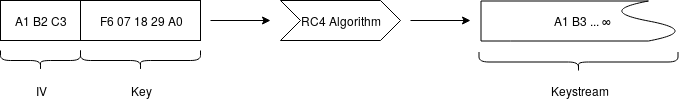
\includegraphics[width=\linewidth]{res/keystream.png}}
\vspace{6px}

A digest (CRC) of the message is then generated to allow to recipient to check for errors.

\vspace{6px}
\centerline{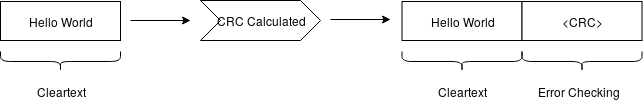
\includegraphics[width=\linewidth]{res/crc.png}}

\newpage
The message and the CRC is then encrypted using the keystream.

\vspace{6px}
\centerline{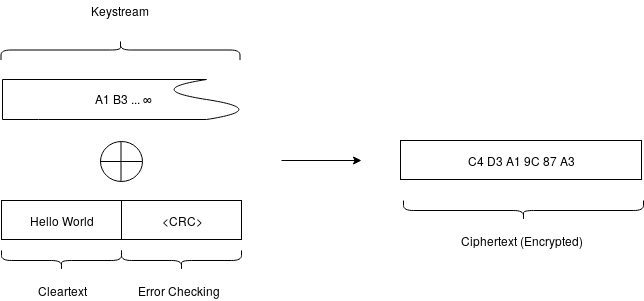
\includegraphics[width=\linewidth]{res/encryption.png}}
\vspace{6px}

Finally, the IV is added so that the recipient can do the entire process in reverse to decrypt to message.

\vspace{6px}
\centerline{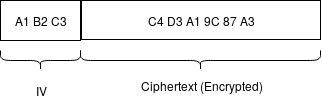
\includegraphics[scale=1.0]{res/header.png}}
\vspace{6px}

\subsection{Weaknesses of WEP}
WEP was superceded by WPA in 2003, and was deprecated due to security concerns in 2004. 

In 2006 a paper was released that showed fundamental flaws in how the WEP standard was designed, allowing attackers to gain access to the key of even the most secure (104-bit) implementations in under 60 seconds \citep{breakingWEP60seconds}. This is particularly damning as the key allows the attacker to decrypt all traffic he or she captures.

\subsection{Business Impact}
The business impact of using WEP with no other mitigations could potentially be very large. Should an attacker come in range of a wi-fi access point they could potentially gather traffic to and from multiple users. If this occurs the massive negative press could potentially bankrupt the business, legal implications notwithstanding. Industry regulators could force the business to close if customer medical or financial information is disclosed.

\newpage
\section{Proposed Solution}
\subsection{VPN}
\subsubsection{Description}
A virtual private network (VPN) allows two private networks to be connected over an unsecured connection by encrypting traffic between two end points. In this case it would add an additional level of encryption that is "tunneled" past WEP. It is routinely utilised by users concerned with privacy and security. If an adversary executes a man-in-the-middle attack, all they will capture is cypher text since the actual message being encrypted by WEP has already been encrypted in the VPN. A diagram of how this could be implemented is included below:

\vspace{6px}
\centerline{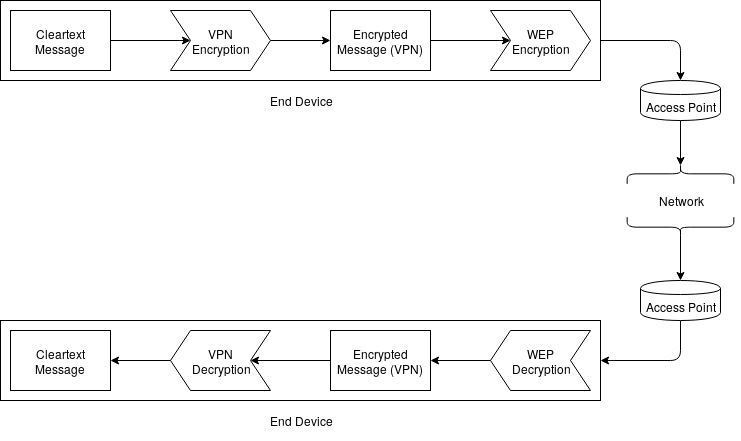
\includegraphics[width=0.7\linewidth]{res/vpn_example.png}}
\vspace{6px}

Should this be implemented as suggested, an attacker will no longer be able to read traffic gathered from the network even if the WEP key is compromised.

\vspace{6px}
\centerline{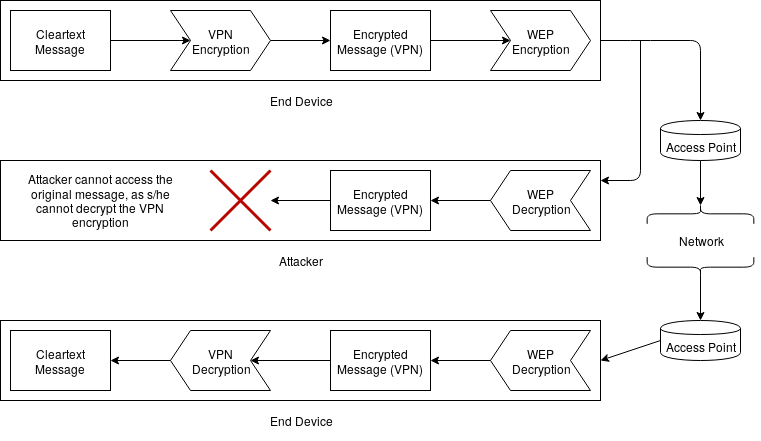
\includegraphics[width=0.7\linewidth]{res/vpn_example_hack.png}}
\vspace{6px}

\subsubsection{IPSEC}
A VPN is not suitable in this case as it connects two trusted networks together over an insecure link, rather than two trusted machines over an insecure network. Instead, the IPSEC protocol should be used as it encrypts traffic between two machines over an untrusted network. It works by taken a packet (a message to be sent over the network), encrypting it, and then encapsulating it within a second packet as the diagram below illustrates:

\vspace{6px}
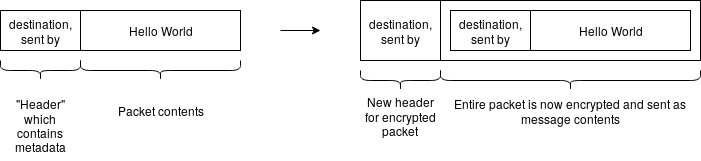
\includegraphics[scale=0.5]{res/ipsec}
\vspace{6px}

This solves the problem of an untrusted network in much the same way a VPN does, as the message can only be decrypted by the intended recipient.

IPSEC is implemented by setting up a database of "security associations" wherein one IP address is associated with another, along with the secret key and the encryption algorithm to be used when they communicate with each other. Policies can then be made using these associations, and stored in a security policy database.

\subsubsection{Implementation}
Since the we are attempting to secure the communications to two endpoints over an untrusted network rather than communication between two networks, peer-to-peer encryption must be used. This is most commonly implemented using IPSEC. This assumes that both machines have operating systems that support IPSEC. Should this not be the case (e.g. when supporting older machines) a custom solution should be used instead.

Below are instructions to set up an example IPSEC VPN:

\begin{enumerate}
\item{Install ipsec-tools on both machines 

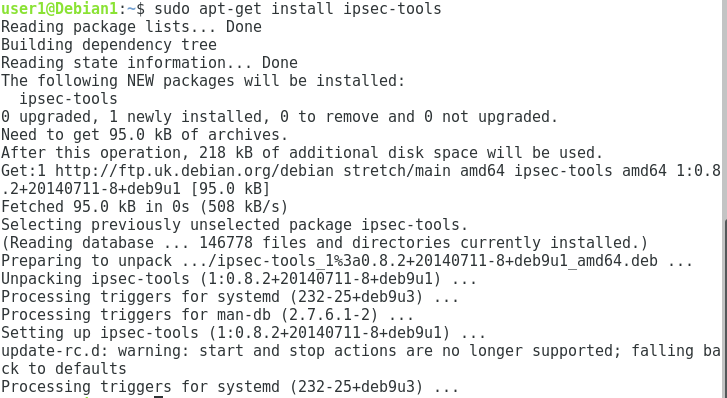
\includegraphics[scale=0.5]{res/install_ipsec_tools}}

\item{Assign machine 1 a static IP address (192.168.1.100)

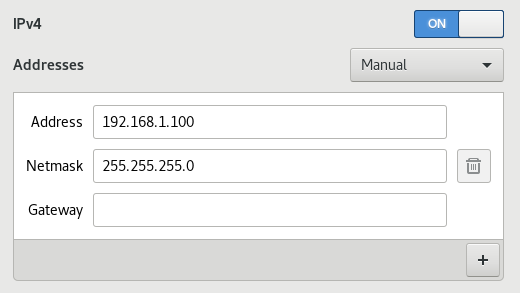
\includegraphics[scale=0.5]{res/machine1/static_ip}}


\item{Assign machine 2 a static IP address (192.168.1.200)

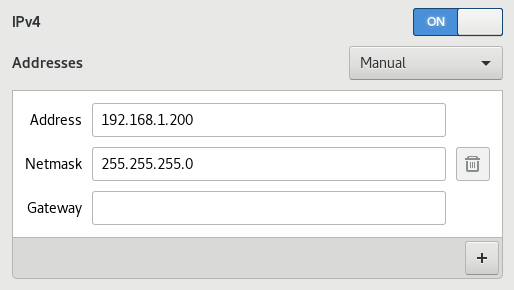
\includegraphics[scale=0.5]{res/machine2/static_ip}}

\newpage
\item{Test connectivity between the two machines

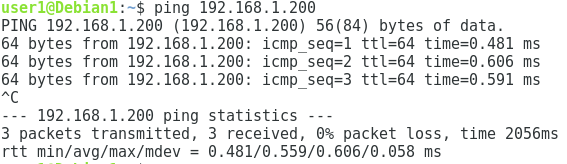
\includegraphics[scale=0.5]{res/machine1/test_connectivity}

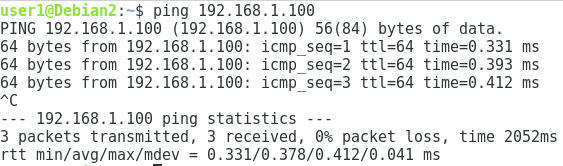
\includegraphics[scale=0.5]{res/machine2/test_connectivity}}

\item{Run the ipsec configuration script on machine 1

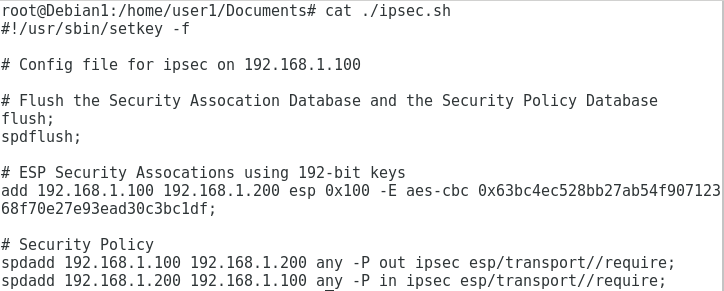
\includegraphics[scale=0.5]{res/machine1/ipsec_config}

The script first deletes any security associations that have been entered in to the database, and any policies that have been made using those associations. Then, it adds a new security association between 192.168.1.100 (machine 1) and 192.168.1.200 (machine 2). The "esp" argument means that the packet should be encrypted, not just signed. The arguments following the -E switch are the encryption method to use (AES-CBC), and the secret key. Finally, two policies are made for incoming and outgoing traffic using the association.
}

\newpage
\item{Run the ipsec configuration script on machine 2

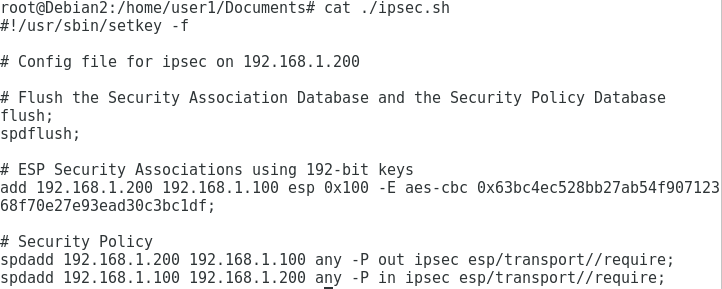
\includegraphics[scale=0.5]{res/machine2/ipsec_config}

This script is almost identical to the script in the previous step, however the direction of travel has been switched in the security policy.
}

\item{Ensure both machines have been configured correctly

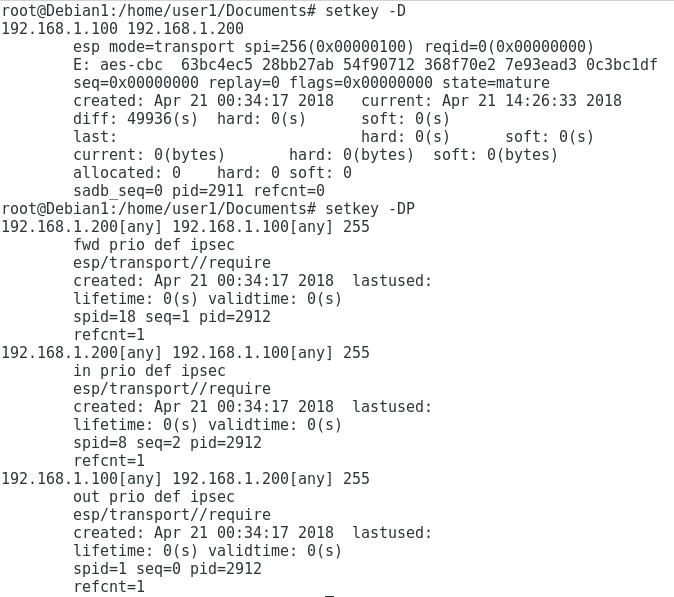
\includegraphics[scale=0.5]{res/machine1/ipsec_running}

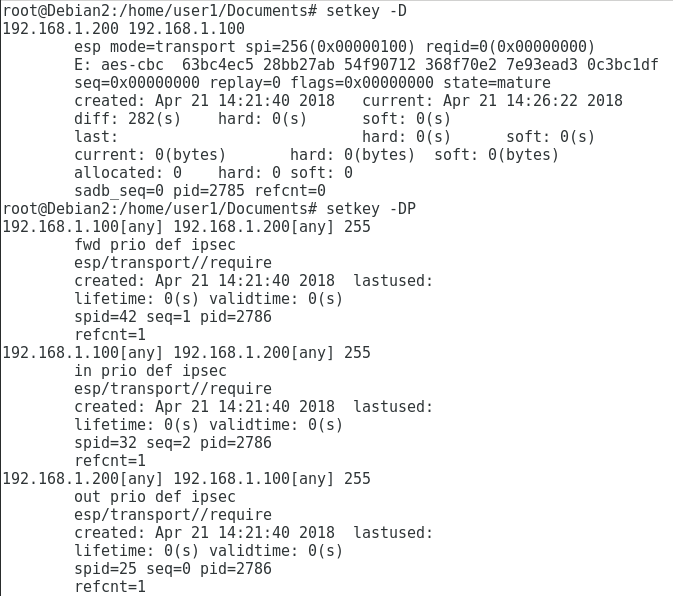
\includegraphics[scale=0.5]{res/machine2/ipsec_running}}

\item{Network traffic between the two machines is now encrypted

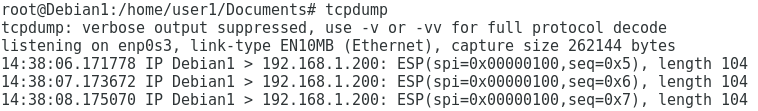
\includegraphics[scale=0.5]{res/machine1/tcpdump}

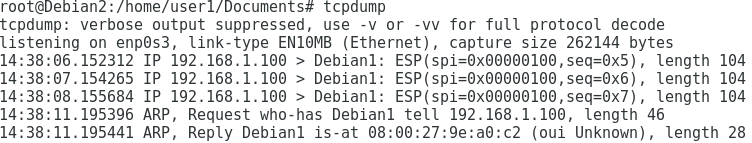
\includegraphics[scale=0.5]{res/machine2/tcpdump}}
\end{enumerate}

\newpage
\subsection{Firewall}
The machine on the network that requires WEP should have every port not in use disabled, and should only be able to communicate with the trusted machine. The firewall should therefore reject all traffic from devices other than 192.168.1.200.

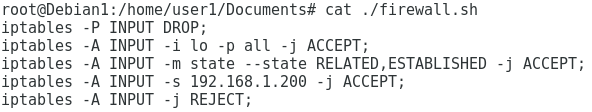
\includegraphics[scale=0.5]{res/machine1/firewall}

\subsection{IDS}
Since ths system is likely to be old (it only supports WEP), it will likely have unpatchable vulnerabilities. Since these cannot be fully mitigated an intrusion detection system (IDS) should be installed on the machine. There are two kinds available, network-based and host-based. If the suggestions given in this report are implemented the network should be a difficult target to attack. Therefore, it is suggested that a host-based detection system be installed to monitor traffic on the machine and report should the machine become compromised. Several commercial products are available. 

\subsection{Update Schedule}
If the machine does not already have a set update schedule, one should be implemented to ensure it remains protected against attacks the manufacturer has created fixes for. If the machine is end-of-life or does not have significant manufacturer support (likely in the case that it only supports WEP), audits should be performed at regular intervals to find and mitigate potential vulnerabilities.

\subsection{Security in depth}
It should be noted that while the mitigations listed above will increase security, they are not a one-time fix. The solutions provided should be reviewed at regular intervals.

\newpage
\section{Ethics}
As security professionals we have a responsibility to use our knowledge only within strict ethical guidelines. While it might seem common sense to some, only attempting to access machines with express permission of the owner as an unbreakable rule is perhaps not as commonplace as it should be. The skills and tools at our disposal should only be used to allow for the effective protection against hostile actors and should not be used to attack themselves.

\subsection{Legal}
There law that governs the majority of activities likely to be undertaken by a penetration tester (in the UK) is the Computer Misuse Act, 1990. It was originally drafted to make unauthorised access to a computer illegal, after two men who gained unauthorised access to the BBC's systems were acquitted after being charged with fraud. It prohibits a person from accessing or attempting to access a system or information contained within a system to which they do not have authorisation to access. From the text;

\begin{enumerate}
\item{A person is guilty of an offense if-}
\begin{enumerate}
\item{he causes a computer to perform any function with intent to secure access to any program or data held in any computer, or to enable any such access to be secured;}
\item{the access he intends to secure, or to enable to be secured, is unauthorised; and}
\item{he knows at the time when he causes the computer to perform the function that that is the case.}
\end{enumerate}
\end{enumerate}

The law also prohibits unauthorised access with intent to commit further offences under section 2 with heavier penalties, as well as denial-of-service attacks under section 3 ("Unauthorised acts with intent to impair, or with recklessness as to impairing, operation of computer, etc." \citep{computermisuseact}).

Obviously, this single act does not cover all ethical issues within the field of information security. There still exists many actions which may be legal but are clearly unethical.

\subsection{Ethical Framework}
The overarching principle that should be adhered to except under specific circumstances when attempting to codify an ethical system is that an individual should never attempt to gain access to anything which is not theirs. This includes things which some may not consider, such as hardware or software which has only been licensed to the end user.

The circumstances in which an individual may attempt to gain access to a system are as follows:

\begin{enumerate}
\item{With the express permission of the owner of the system;}
\item{With the express permission of a maintainer of the system, acting under the authority of the owner;}
\item{Within the terms set under a legally binding engagement document which outlines which systems a person may attempt to gain access to, who is liable for any damage caused and what methods of attack may be used.}
\end{enumerate}

It is hard to imagine a scenario in which an unethical action could be taken when following this framework (at least, in the context of information security). Penetration tests, for example, fall under section 3. Bug bounties fall under section 2.

\subsection{Professional Standards}
There are many professional standards that a person may follow in an information security career. Two of the most desirable certifications have been detailed below:

\subsubsection{Certified Information Systems Security Professional}
The Certified Information Systems Security Professional (CISSP) certification is a globally recognised professional standard that is ratified by the International Information System Security Certification Consortium, known also as $(isc)^2$. It requires candidates to pass an examination, have at least 5 years of full-time information security employment, answer questions about their criminal history and accept the CISSP code of ethics \citep{CISSPethics}.

\subsubsection{Offensive Security Certified Professional}
Seen by many as the "gold standard" for information security professionals, the Offensive Security Certified Professional (OSCP) certification aims to closely mirror a real-world engagement. It is offered by Offensive Security, the company behind the Kali distribution of Linux (one of the most widely used collection of tools for information security professionals). It is renowned for being extremely difficult, as candidates are expected to gain access to an unfamiliar system, document the process used and prove that access was gained by recording "flags" which change per-exam.

\newpage
\bibliography{citations}

\end{document}